%%
%% Automatically generated file from DocOnce source
%% (https://github.com/hplgit/doconce/)
%%
%%


%-------------------- begin preamble ----------------------

\documentclass[%
oneside,                 % oneside: electronic viewing, twoside: printing
final,                   % draft: marks overfull hboxes, figures with paths
10pt]{article}

\listfiles               %  print all files needed to compile this document
\usepackage{mathtools}
\usepackage{relsize,makeidx,color,setspace,amsmath,amsfonts,amssymb}
\usepackage[table]{xcolor}
\usepackage{bm,ltablex,microtype}
\usepackage{float}
\usepackage[pdftex]{graphicx}
\usepackage{epstopdf}
\usepackage{verbatim}

\usepackage{fancyvrb} % packages needed for verbatim environments

\usepackage[T1]{fontenc}
%\usepackage[latin1]{inputenc}
\usepackage{ucs}
\usepackage[utf8x]{inputenc}
\usepackage[english]{babel}
\usepackage{lmodern}         % Latin Modern fonts derived from Computer Modern

% Hyperlinks in PDF:
\definecolor{linkcolor}{rgb}{0,0,0.4}
\usepackage{hyperref}
\hypersetup{
    breaklinks=true,
    colorlinks=true,
    linkcolor=linkcolor,
    urlcolor=linkcolor,
    citecolor=black,
    filecolor=black,
    %filecolor=blue,
    pdfmenubar=true,
    pdftoolbar=true,
    bookmarksdepth=3   % Uncomment (and tweak) for PDF bookmarks with more levels than the TOC
    }
%\hyperbaseurl{}   % hyperlinks are relative to this root

\setcounter{tocdepth}{2}  % levels in table of contents



% prevent orhpans and widows
\clubpenalty = 10000
\widowpenalty = 10000

% --- end of standard preamble for documents ---


% insert custom LaTeX commands...

\raggedbottom
\makeindex
\usepackage[totoc]{idxlayout}   % for index in the toc
\usepackage[nottoc]{tocbibind}  % for references/bibliography in the toc

%-------------------- end preamble ----------------------

\begin{document}

% matching end for #ifdef PREAMBLE

\newcommand{\exercisesection}[1]{\subsection*{#1}}


% ------------------- main content ----------------------



% ----------------- title -------------------------

\thispagestyle{empty}

\begin{center}
{\LARGE\bf
\begin{spacing}{1.25}
PHYS 905 - Project 3
\end{spacing}
}
\end{center}

% ----------------- author(s) -------------------------

\begin{center}
{\bf Terri Poxon-Pearson}
\end{center}

    
% ----------------- end author(s) -------------------------

% --- begin date ---
\begin{center}
March 27, 2017
\end{center}
% --- end date ---

\vspace{1cm}

INSERT ABSTRACT HERE

\tableofcontents
 
\section{Introduction}

Differential equations are one of the most important tools that physicists have for expressing physical laws.  From Maxwell's equations to Einstein's field question in general relativity, differential equations are the mathematical language for almost every physical process.  Outside of physics, differential equations can be used describe systems in finance, ecosystems, and medicine.  The ubiquity of these relationships demands that we have efficient and accurate algorithms for solving these problems.

In this project we will focus on one of the earliest differential equations, first expressed by Newton \cite{LectureNotes}.  Newton's Second law is an example of an ordinary differential equation, where ordinary refers to the fact that it is a function of independent variable and its derivatives.  Once the differential equation is solved analytically, initial values must be provided to find the exact solution.  When we solve these problems numerically, we will provide initial values to begin the solver. 

Specifically in this project we will be simulating the motion of the planets in the solar system.  We will explore two different Algorithms for solving initial value ODEs: the Euler Algorithm and the Velocity Verlet Algorithm.  We will begin by looking at the simpler two body, Sun-Earth system and expand this to the Sun-Earth-Jupiter system and, eventually, the entire solar system.  The solar system will be implemented using Object Oriented (OO) programming in order to take advantage of the repetitive structure of the ODEs.  Initial conditions for this system come from data provided by NASA's Jet Propulsion Laboratory.  Finally, we will end with some remarks and conclusions.

\section{Methods}

\subsection{Newton's Equations for the Earth Sun System}

The motion of the planets are dictated by the gravitational force which is given by
\[
F_G=\frac{GM_{\odot}M_{\mathrm{Earth}}}{r^2},
\]
where $M_{\odot}$ is the mass of the Sun and $M_{\mathrm{Earth}}$ is the mass of the Earth.  $G$ is the universal gravitational constant and $r$ is the distance between the center of mass of the Earth and the Sun.  The Sun's mass is over 300,000 times the mass of the Earth so, for our model, we can safely neglect any motion of the Sun.  Newton's second law states 
\[
\frac{d^2x}{dt^2}=\frac{F_{G,x}}{M_{\mathrm{Earth}}},
\]
and 
\[
\frac{d^2y}{dt^2}=\frac{F_{G,y}}{M_{\mathrm{Earth}}},
\]
where $F_{G,x}$ and $F_{G,y}$ are the $x$ and $y$ components of the gravitational force.  There is an analogous equation for z, but the orbit of the earth is, to good approximation, confined to a plane so we will neglect this for now.  If we substitute in the relationship for force and make the substitution that $x=r cos(\theta)$ and $y=r sin(\theta)$, we are left with
\[
\frac{d^2x}{dt^2}=-\frac{GM_{\odot}x}{r^3},
\]
and 
\[
\frac{d^2y}{dt^2}=-\frac{GM_{\odot}y}{r^3},
\]

where $ r=\sqrt{x^2+y^2} $.  Now we want to rewrite these equations as first order differential equations.  We do this by making the substitution that velocity is the first derivative of position.  This substitution leaves us with four, first order, ODEs:

\[
\frac{dx}{dt}=v_x
\]
\[
\frac{dy}{dt}=v_y
\]
\[
\frac{dv_x}{dt}=-\frac{GM_{\odot}x}{r^3}
\]
\[
\frac{dv_y}{dt}=-\frac{GM_{\odot}y}{r^3}.
\]

Finally, we can clean up these equations by our choice of units and a clever substitution.  The natural unit for this system is the Astronomical Unit (AU) which is the average distance between the Sun and Earth.  We will use years as our unit of time.  For circular motion, we know that 
\[
F_G= \frac{M_{\mathrm{Earth}}v^2}{r}=\frac{GM_{\odot}M_{\mathrm{Earth}}}{r^2},
\]
where $v$ is the velocity of Earth.  If the radius of the Earth's orbit is 1AU, then the velocity of the Earth is $\pi 1AU^2$.  Substitution this in, the equation above can be solved to show that 
\[
v^2r=GM_{\odot}=4\pi^2\mathrm{AU}^3/\mathrm{yr}^2.
\]

Making this final substitution, the ODEs which we must solve are

\[
\frac{dx}{dt}=v_x
\]
\[
\frac{dy}{dt}=v_y
\]
\[
\frac{dv_x}{dt}=-\frac{4 \pi^2 x}{r^3}
\]
\[
\frac{dv_y}{dt}=-\frac{4 \pi^2 y}{r^3}.
\]


\subsection{Euler's Method}

The first method we will implement for solving the Sun-Earth system is Euler's Method.  This method is derived from a Taylor expansion which can be expressed as 

\[
f(x+h) = \sum_{i=0}^{\infty} \frac{h^i}{i!}f^{(i)}(x)
\]

where $f^{(i)}$ is the $i$th derivative and h is a step in the $x$ variable.  If we keep only the first two terms, we are left with

\[
f(x+h) = f(x) + hf^{(1)} +O(h^2).
\]

Applying this relationship to our four differential equation, the algorithm for Euler's method is

\[
x_{i+1} = x_i +v_{xi} + O(h^2)
\]
\[
y_{i+1} = y_i +v_{yi} + O(h^2)
\]
\[
v_{x_i+1} = v_{x_i} -\frac{4 \pi^2}{r_i^3}x_i h + O(h^2)
\]
\[
v_{y_i+1} = v_{y_i} -\frac{4 \pi^2}{r_i^3}y_i h + O(h^2).
\]

In this case, h is a step in time so $h=\frac{t_{max}-t_{min}}{N}$ where $N$ is the number of time steps used.

\subsection{Velocity Verlet Algorithm}

The Verlet method also begins with a Taylor expansion, this time to second order, gving us

\[
x(t+h) = x(t)+hx^{(1)}(t)+\frac{h^2}{2}x^{(2)}(t) + O(h^3).
\]

We know from Newton's law that the second derivative position is equatl to the acceleration.  We can then add the cooresponding equation for the Taylor expansion of $x(t-h)$

\[
x(t-h) = x(t)-hx^{(1)}(t)+\frac{h^2}{2}x^{(2)}(t) + O(h^3).
\]

After this addition and our usual discritization of the expressions, we obtain

\[
x_{i+1}=2x_i -x_{i-1}+h^2x_i^{(2)}+O(h^4).
\]

This expression is nice because the turncation error in position goes as $O(h^4)$, but it also has an obvious flaw.  If we set an initial value for $x_0$, it is unclear how to handle the $x_{i-1}$ term.  This means the position is not "self-starting."  We can deal with this by introducing, instead, the Velocity Verlet method.

We can start again with 2nd order Taylor expansions for position and velocity

\[
x_{i+1} =x_i +hx_i^{(1)}+\frac{h^2}{2}x_i^{(2)}+O(h^3)
\]
and
\[
v_{i+1} =v_i +hv_i^{(1)}+\frac{h^2}{2}v_i^{(2)}+O(h^3).
\]

We know that the first derivative of position is velocity and Newton's law gives us an expression for the first derivative of velocity and the second derivative of position

\[
v_i^{(1)}=\frac{d^2x}{dt^2}|_i=\frac{f(x_i,t_i)}{m}
\]

Newton's law, however, does not provide an expression for the second derivative of velocity, but we can obtain this through the expanding the first derivative of velocity

\[
v_{i+1}^{(1)}=v_i^{(1)} + hv_i^{(2)}+O(h^2).
\]

Solving this expression for $v_i^{(2)}$ gives us a value to plug into our Taylor expansion.  After making that substitution, our final Velocity Verlet algorithm expressions are

\[
x_{i+1} =x_i +hv_i+\frac{h^2}{2}v_i^{(1)}+O(h^3)
\]
and
\[
v_{i+1} =v_i +\frac{h}{2} \big(v_{i+1}^{(1)}+v_i^{(1)} \big)+O(h^3).
\]

These expressions are self-starting, but require the position at time $t_{i+1}$ is calculated becfore the velocity at that point can be calculated.

\subsection{Expanding Equations to Solar System}

It is fairly straightforward to expand the expressions for the Sun-Earth system to include the entire Solar System.  As an example, we can think about adding Jupiter to the system, giving us a three-body problem.  Jupiter is a natural choice becuase it is the heaviest planet in the solar syster, about 1000 times smaller than the Sun.  The gravitational force between the Earth and Jupiter is

\[
F_{\mathrm{Earth-Jupiter}}=\frac{GM_{\mathrm{Jupiter}}M_{\mathrm{Earth}}}{r_{\mathrm{Earth-Jupiter}}^2},
\]

We can apply the same transformations as before and obtain the following expression for the motion of the Earth

\[
\frac{dv_x^E}{dt}=-\frac{G M_{\odot}}{r^3}x_E - \frac{G M_{J}}{r^3_{EJ}}(x_E-x_J).
\]

If we normalize everything to the orbit and mass of the earth, we obtain

\[
\frac{dv_x^E}{dt}=-\frac{4 \pi^2}{r^3}x_E - \frac{4 \pi^2 M_J/M_{\odot}}{r^3_{EJ}}(x_E-x_J).
\]

There is an analogous equation for motion in the y and z position.  In this report we seperately study the Earth-Sun, Sun-Earth-Jupiter, and Solar Systems.  To expand these expressions to the entire solar system, one just needs to add an additional force term corresponding to each two body interaction.  These forces can all be summed into one total force and used in the same Velocity Verlet expressions from the previous section.  The masses and distances to the Sun for the solar system are given in the table below.

\begin{quote}
\begin{tabular}{ccc}
\hline
\multicolumn{1}{c}{ Planet } & \multicolumn{1}{c}{ Mass in kg } & \multicolumn{1}{c}{ Distance to  sun in AU } \\
\hline
Earth   & $M_{\mathrm{Earth}}=6\times 10^{24}$ kg     & 1AU                    \\
Jupiter & $M_{\mathrm{Jupiter}}=1.9\times 10^{27}$ kg & 5.20 AU                \\
Mars    & $M_{\mathrm{Mars}}=6.6\times 10^{23}$ kg    & 1.52 AU                \\
Venus   & $M_{\mathrm{Venus}}=4.9\times 10^{24}$ kg   & 0.72 AU                \\
Saturn  & $M_{\mathrm{Saturn}}=5.5\times 10^{26}$ kg  & 9.54 AU                \\
Mercury & $M_{\mathrm{Mercury}}=3.3\times 10^{23}$ kg & 0.39 AU                \\
Uranus  & $M_{\mathrm{Uranus}}=8.8\times 10^{25}$ kg  & 19.19 AU               \\
Neptun  & $M_{\mathrm{Neptun}}=1.03\times 10^{26}$ kg & 30.06 AU               \\
Pluto   & $M_{\mathrm{Pluto}}=1.31\times 10^{22}$ kg  & 39.53 AU               \\
\hline
\end{tabular}
\end{quote}

\section{Code and Implementation}

All of the programs, results, and benchmarks for this work can be found in my GIT repository ( https://github.com/poxonpea/PHYS905 ).  All codes for this project were written in FORTRAN.

\subsection{Implementing Euler and Verlet Algorithms}

The code containing the most important elements of Euler's method for the Sun-Earth is shown below.

\begin{figure}[H]\label{fig:eulercode}
  \centering
    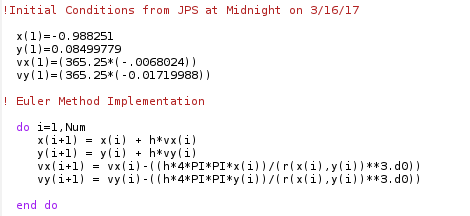
\includegraphics[width=0.8\textwidth]{EulerCode.png}
    \caption{The code used to implement Euler's method for the Sun Earth system.}
\end{figure}

While this algorithm is simple, it is also unstable.  The plot below shows the trajectory of the earth over 10 years in 1000 time steps using initial conditions from the Jet Propulsion Labratory \cite{JPL} at midnight on March 16,2017.

\begin{figure}[H]\label{fig:eulerplot}
  \centering
    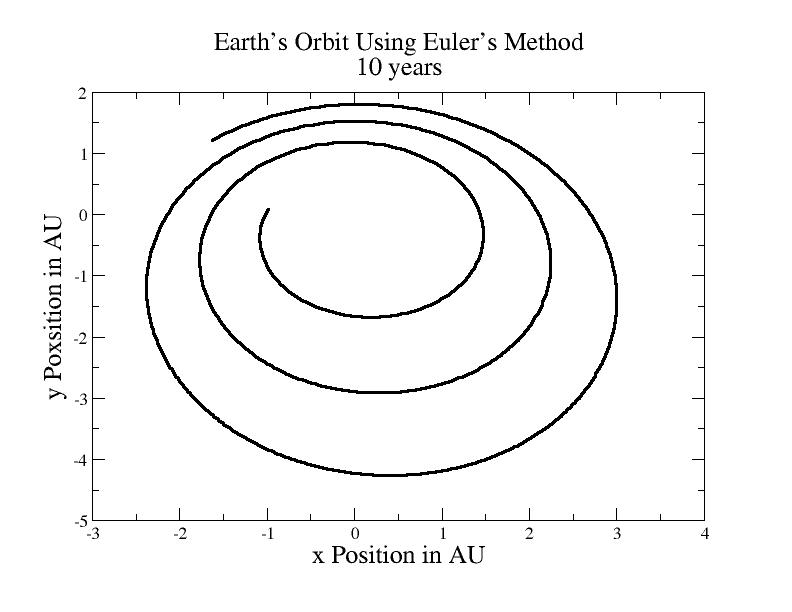
\includegraphics[width=1.0\textwidth]{Euler.jpg}
    \caption{The trajectory of the Earth in the Sun-Earth system produced by Euler's method}
\end{figure}

Almost immediately, the trajectory begins to spin out away from the Sun.  Because of this, there is no point pursuing this method for larger systems.  Instead, we will use the Velocity Verlet method.  The code containing the most important elements of te Velocity Verlet method for the Sun-Earth is shown below.

\begin{figure}[H]\label{fig:velcode}
  \centering
    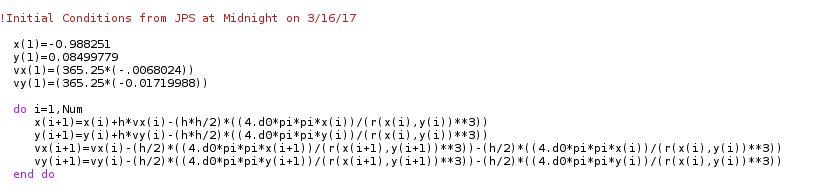
\includegraphics[width=1.0\textwidth]{VelCode.png}
    \caption{The code used to implement the Velocity Verlet method for the Sun Earth system.}
\end{figure}

The plot below shows the trajectory of the earth over 10 years in 1000 time steps using initial conditions from the Jet Propulsion Labratory at midnight on March 16,2017.

\begin{figure}[H]\label{fig:velrplot}
  \centering
    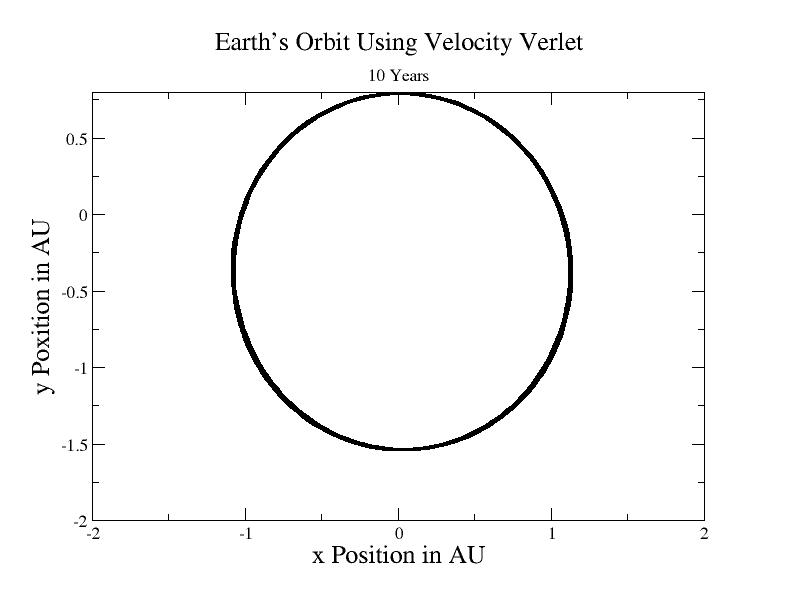
\includegraphics[width=1.0\textwidth]{velverearth.jpg}
    \caption{The trajectory of the Earth in the Sun-Earth system produced by the Velocity Verlet method}
\end{figure}

Unlike Euler's method, the Velocity Verlet algorithm produces a stable, almost circular orbit.  We will use this algorithm to extend our code to the Sun-Earth-Jupiter and Solar Stystems.  Because all of the equations for this system follow a similar format, we will switch to an OO structure for our code, which will be discussed in more detail in the following section. 

\subsection{Object Oriented Code}

\subsection{Tests of Code}

\section{Results and Discussion}


\subsection{Escape Velocity of the Sun-Earth System}

If an object's kinetic energy exceeds the potential energy keeping it in orbit, it can escape from the system.  This escape velocity can be found by

\[
-\frac{G m_1 M_2}{R}=\frac{1}{2}m_1 v^2
\]
so 
\[
v_{esc}=\sqrt{\frac{2GM_2}{R}}.
\]

The normal orbital velocity can be found by setting the gravitational force equal to the centripetal force.  Solving this leaves us with an orbital velocity of $v_{orb}=\sqrt{\frac{GM_2}{R}}$ so that

\[
v_{escape}=\sqrt{2}v_{orbit}.
\]

For the Earth, the velocity is $2 \pi$ AU/year, so the escape velocity should be roughtly $\sqrt{2}2\pi$ AU/year.

\subsection{The Three Body Problem}

\subsection{Solar System Model}


\section{Conclusions}


\section{Appendices}

\subsection{Appendix A} \label{A}



\begin{comment}

\begin{figure}[H]\label{fig:compzoom}
  \centering
    \includegraphics[width=1.2\textwidth]{compzoom.eps}
    \caption{A zoomed in view of the convergence to the exact solution}
\end{figure}

\begin{center} 
\begin{tabular}{ |c|c|c|c| }
\hline
Size of Matrix ($10^n$) & General & Tailored & LU \\
\hline
1& 3.00 E -6 & 3.00 E -6 & 2.40 E -5\\ 
2 & 4.00 E -6 & 4.00 E -6 & 1.71 E -3 \\ 
3 & 3.90 E -5 & 1.90 E -5 & 1.93\\ 
4 & 3.79 E -4 & 2.09 E -4 & N/A\\ 
5 & 3.38 E -3 & 1.51 E -3  & N/A\\ 
6 & 2.87 E -2 & 1.53 E -2 & N/A\\ 
7 & 3.16 E -1 & 1.73 E -1& N/A\\ 
\hline
\end{tabular}
\label{table:test}
\end{center}

\end{comment}

\begin{thebibliography}{9}

\bibitem{LectureNotes} 
Hjorth-Jensen, Mortehn. 
Computational Physics, Lecture Notes Fall 2015. 
August 2015.

\bibitem{JPL} 
Jet Propulsion Laboratory .
HORIZONS Web-Interface. 
http://ssd.jpl.nasa.gov/horizons.cgi.


\end{thebibliography}



% ------------------- end of main content ---------------

\end{document}

